%=====================================================================
%  SHARED PREAMBLE — Quantitative Reasoning LAB 413 Beamer theme
%  Paste this block VERBATIM at the top of every LabN_beamer.tex
%  (keep each deck self-contained; do NOT \input this file).
%  Compile: pdflatex LabN_beamer.tex   (run twice for footline counters)
%=====================================================================
\documentclass[aspectratio=169,11pt]{beamer}

\usepackage[utf8]{inputenc}
\usepackage[T1]{fontenc}
\usepackage{lmodern}
\usepackage{amsmath,amssymb}
\usepackage{graphicx}
\usepackage{booktabs}
\usepackage{tcolorbox}
\tcbuselibrary{skins}

\usetheme{default}
\usecolortheme{default}
\useinnertheme{circles}

\definecolor{qrnavy}{RGB}{20,44,90}
\definecolor{qrblue}{RGB}{38,80,150}
\definecolor{qrgray}{RGB}{90,95,105}
\definecolor{qrlight}{RGB}{234,239,247}
\definecolor{qrred}{RGB}{190,60,60}

\setbeamercolor{structure}{fg=qrnavy}
\setbeamercolor{frametitle}{fg=white,bg=qrnavy}
\setbeamercolor{title}{fg=qrnavy}
\setbeamercolor{block title}{fg=white,bg=qrblue}
\setbeamercolor{block body}{bg=qrlight}
\setbeamercolor{itemize item}{fg=qrblue}
\setbeamercolor{itemize subitem}{fg=qrblue}
\setbeamerfont{frametitle}{series=\bfseries}
\setbeamertemplate{navigation symbols}{}

\setbeamertemplate{frametitle}{%
  \nointerlineskip
  \begin{beamercolorbox}[wd=\paperwidth,ht=3.2ex,dp=1.2ex,leftskip=0.3cm]{frametitle}%
    \strut\insertframetitle\strut
  \end{beamercolorbox}%
}

% Footline: course | lab N | slide number  (edit "Lab N" per deck)
\newcommand{\labnum}{Lab 5}   % <-- SET THIS to the lab number, e.g. \renewcommand{\labnum}{Lab 3}
\setbeamertemplate{footline}{%
  \leavevmode%
  \hbox{%
    \begin{beamercolorbox}[wd=.5\paperwidth,ht=2.4ex,dp=1ex,leftskip=.3cm]{author in head/foot}%
      \usebeamerfont{author in head/foot}\color{qrgray}\small Quantitative Reasoning -- LAB 413%
    \end{beamercolorbox}%
    \begin{beamercolorbox}[wd=.5\paperwidth,ht=2.4ex,dp=1ex,rightskip=.3cm]{title in head/foot}%
      \usebeamerfont{title in head/foot}\color{qrgray}\small\hfill \labnum \quad\insertframenumber\,/\,\inserttotalframenumber%
    \end{beamercolorbox}}%
}

% Number badge (01, 02, ...) used on concept slides:  \numbadge{01}
\newtcbox{\numbadge}{on line,boxsep=2pt,left=4pt,right=4pt,top=2pt,bottom=2pt,
  colback=qrnavy,colframe=qrnavy,fontupper=\bfseries\color{white},arc=2pt}

% Key-concepts callout:  \begin{keybox} ... \end{keybox}   or  \begin{keybox}[Scenario] ...
\newtcolorbox{keybox}[1][Key Concepts]{colback=qrlight,colframe=qrnavy,
  fonttitle=\bfseries,title={#1},coltitle=white,arc=2pt,left=4pt,right=4pt,
  top=3pt,bottom=3pt,boxrule=0.6pt}

%---------------------------------------------------------------------
%  Title data
%---------------------------------------------------------------------
\title{\bfseries Probability \& Sampling Distributions}
\subtitle{Week 6 Recap \textbullet\ Lab 5}
\author{Instructor: Subin Na}
\institute{Quantitative Reasoning -- LAB 413}
\date{October 1, 2025}

\begin{document}

%---------------------------------------------------------------------
%  Title slide
%---------------------------------------------------------------------
{\setbeamertemplate{footline}{}
\begin{frame}
  \vfill
  {\color{qrgray}\small Quantitative Reasoning -- LAB 413}\\[0.6em]
  {\usebeamerfont{title}\color{qrnavy}\huge\bfseries Probability\\[0.15em]\& Sampling Distributions\par}
  \vspace{0.4em}
  {\color{qrblue}\large Week 6 Recap \ \textbullet\ \ Lab 5}\par
  \vspace{1.6em}
  {\color{qrgray} Instructor: \textbf{Subin Na} \hfill October 1, 2025}
  \vfill
\end{frame}
}

%---------------------------------------------------------------------
%  Today's Plan
%---------------------------------------------------------------------
\begin{frame}{Today's Plan}
  \begin{columns}[T]
    \begin{column}{0.5\textwidth}
      \textbf{\color{qrnavy}1. Quick Recap}
      \begin{itemize}
        \item Why Probability Matters
        \item Essential Probability Rules
        \item Random Variables
        \item Statistical Inference
      \end{itemize}
    \end{column}
    \begin{column}{0.5\textwidth}
      \phantom{\textbf{x}}
      \begin{itemize}
        \item Sampling Distributions
        \item Key Theorems
      \end{itemize}
      \vspace{0.8em}
      \textbf{\color{qrnavy}2. RStudio Practice}
    \end{column}
  \end{columns}
\end{frame}

%---------------------------------------------------------------------
%  01 Why Probability Matters
%---------------------------------------------------------------------
\begin{frame}{\numbadge{01}\ \ Why Probability Matters}
  \begin{keybox}[The Problem]
    How do we know if our estimates are \emph{``real''} or just due to random chance?
  \end{keybox}
  \vspace{0.4em}
  \textbf{\color{qrnavy}The Solution.} Probability helps us understand random
  variability and uncertainty.
  \vspace{0.5em}
  \begin{columns}[T]
    \begin{column}{0.48\textwidth}
      \begin{tcolorbox}[colback=white,colframe=qrnavy,arc=3pt,halign title=center,
        title=\bfseries Probability,coltitle=white,colbacktitle=qrnavy]
        \centering Know population distribution $\rightarrow$ predict sample outcomes
      \end{tcolorbox}
    \end{column}
    \begin{column}{0.48\textwidth}
      \begin{tcolorbox}[colback=white,colframe=qrnavy,arc=3pt,halign title=center,
        title=\bfseries Statistical Inference,coltitle=white,colbacktitle=qrnavy]
        \centering Have sample data $\rightarrow$ infer population characteristics
      \end{tcolorbox}
    \end{column}
  \end{columns}
\end{frame}

%---------------------------------------------------------------------
%  02 Essential Probability Rules  (RECREATE math)
%---------------------------------------------------------------------
\begin{frame}{\numbadge{02}\ \ Essential Probability Rules}
  \textbf{\color{qrnavy}Fundamental Rules}
  \vspace{0.6em}
  \begin{align*}
    \textbf{Range:} &\quad 0 \le P(A) \le 1\\[0.3em]
    \textbf{Total Probability:} &\quad P(S) = 1\\[0.3em]
    \textbf{Complement Rule:} &\quad P(\text{not } A) = 1 - P(A)\\[0.3em]
    \textbf{Addition Rule:} &\quad P(A \text{ or } B) = P(A) + P(B) - P(A \text{ and } B)\\[0.3em]
    \textbf{Multiplication Rule:} &\quad P(A \text{ and } B) = P(A) \times P(B \mid A)
  \end{align*}
\end{frame}

%---------------------------------------------------------------------
%  03 Random Variables  (EMBED discrete-vs-continuous figure)
%---------------------------------------------------------------------
\begin{frame}{\numbadge{03}\ \ Random Variables}
  \begin{keybox}[Definition]
    A random variable \textbf{assigns numeric values to outcomes}.
  \end{keybox}
  \vspace{0.3em}
  \begin{columns}[T]
    \begin{column}{0.42\textwidth}
      \textbf{\color{qrnavy}Two types}
      \begin{itemize}
        \item \textbf{Discrete:} countable values \\(e.g., number of heads in coin
              flips, survey responses)
        \item \textbf{Continuous:} any real value \\(e.g., height, income)
      \end{itemize}
    \end{column}
    \begin{column}{0.56\textwidth}
      \centering
      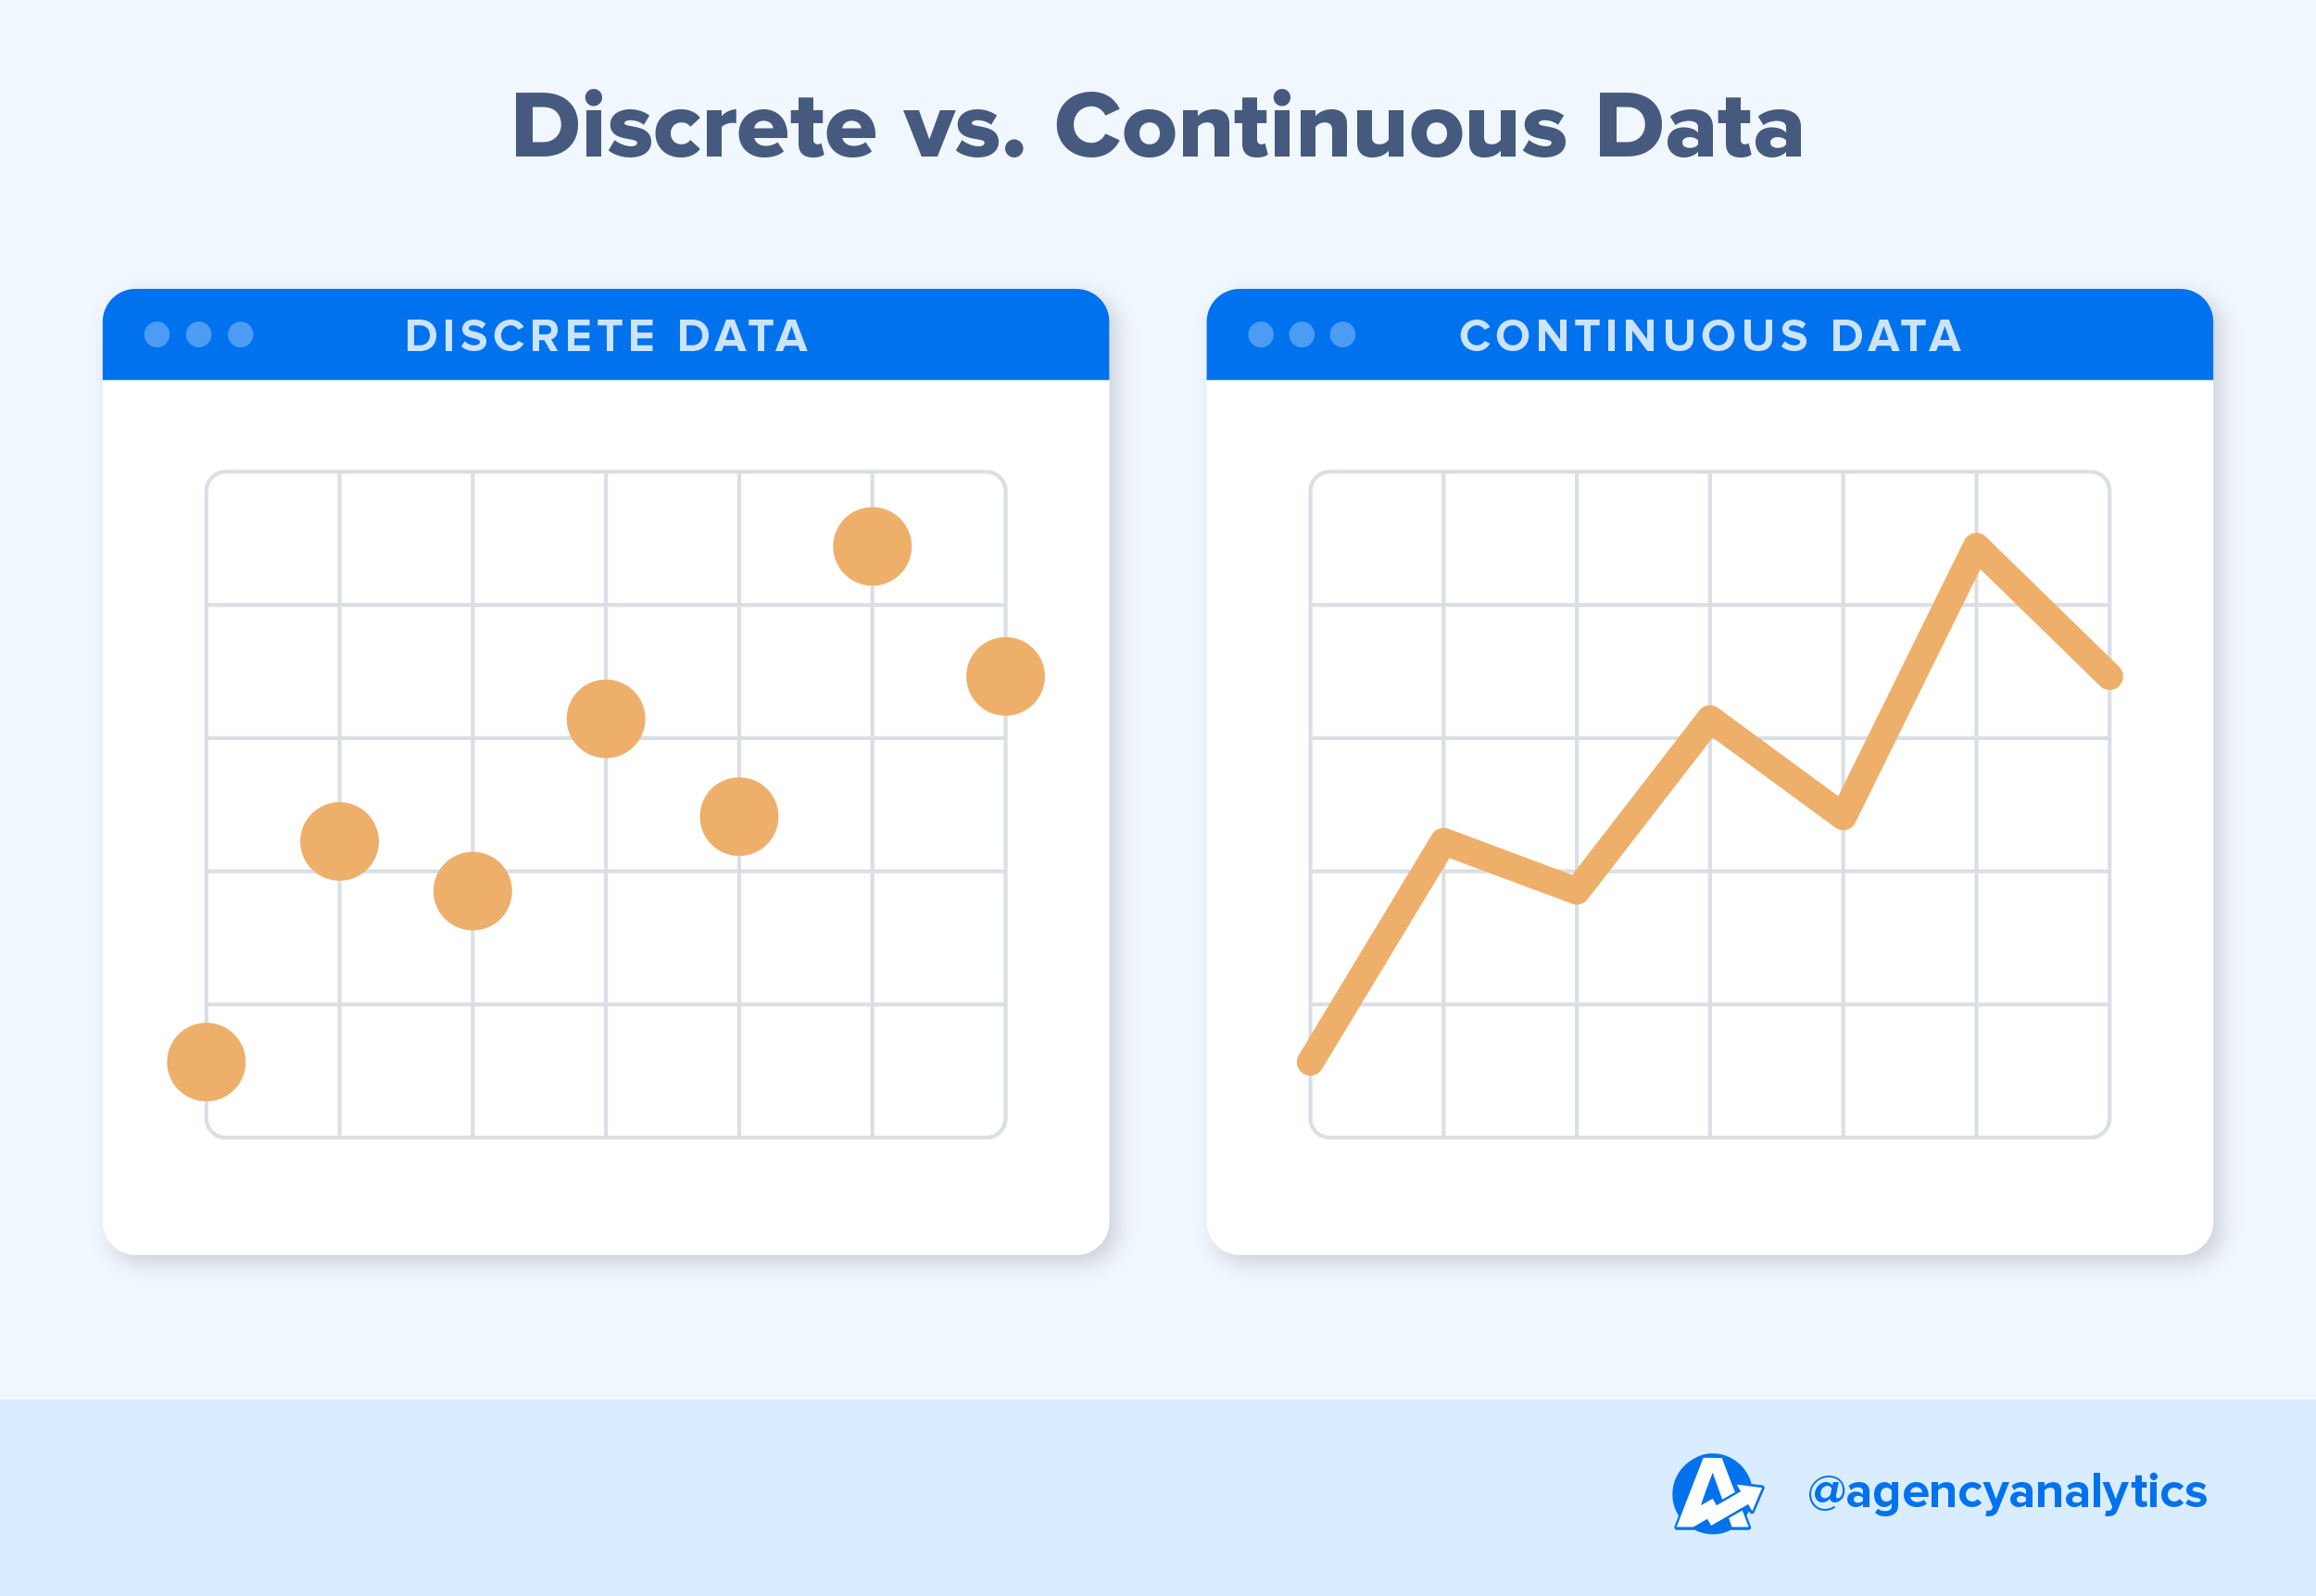
\includegraphics[width=\textwidth]{figures/s05_1_6.8x3.7.png}
    \end{column}
  \end{columns}
\end{frame}

%---------------------------------------------------------------------
%  04 Statistical Inference  (EMBED samples -> sampling distribution)
%---------------------------------------------------------------------
\begin{frame}{\numbadge{04}\ \ Statistical Inference}
  \begin{columns}[T]
    \begin{column}{0.5\textwidth}
      \textbf{\color{qrnavy}Goal.} Use sample statistics to estimate population parameters.
      \vspace{0.5em}
      \begin{itemize}
        \item \textbf{Parameter:} unknown population characteristic ($\mu$, $\sigma$)
        \item \textbf{Statistic:} sample-based estimate ($\bar{x}$, $s$)
        \item \textbf{Sampling Distribution:} how statistics vary across samples
      \end{itemize}
    \end{column}
    \begin{column}{0.5\textwidth}
      \centering
      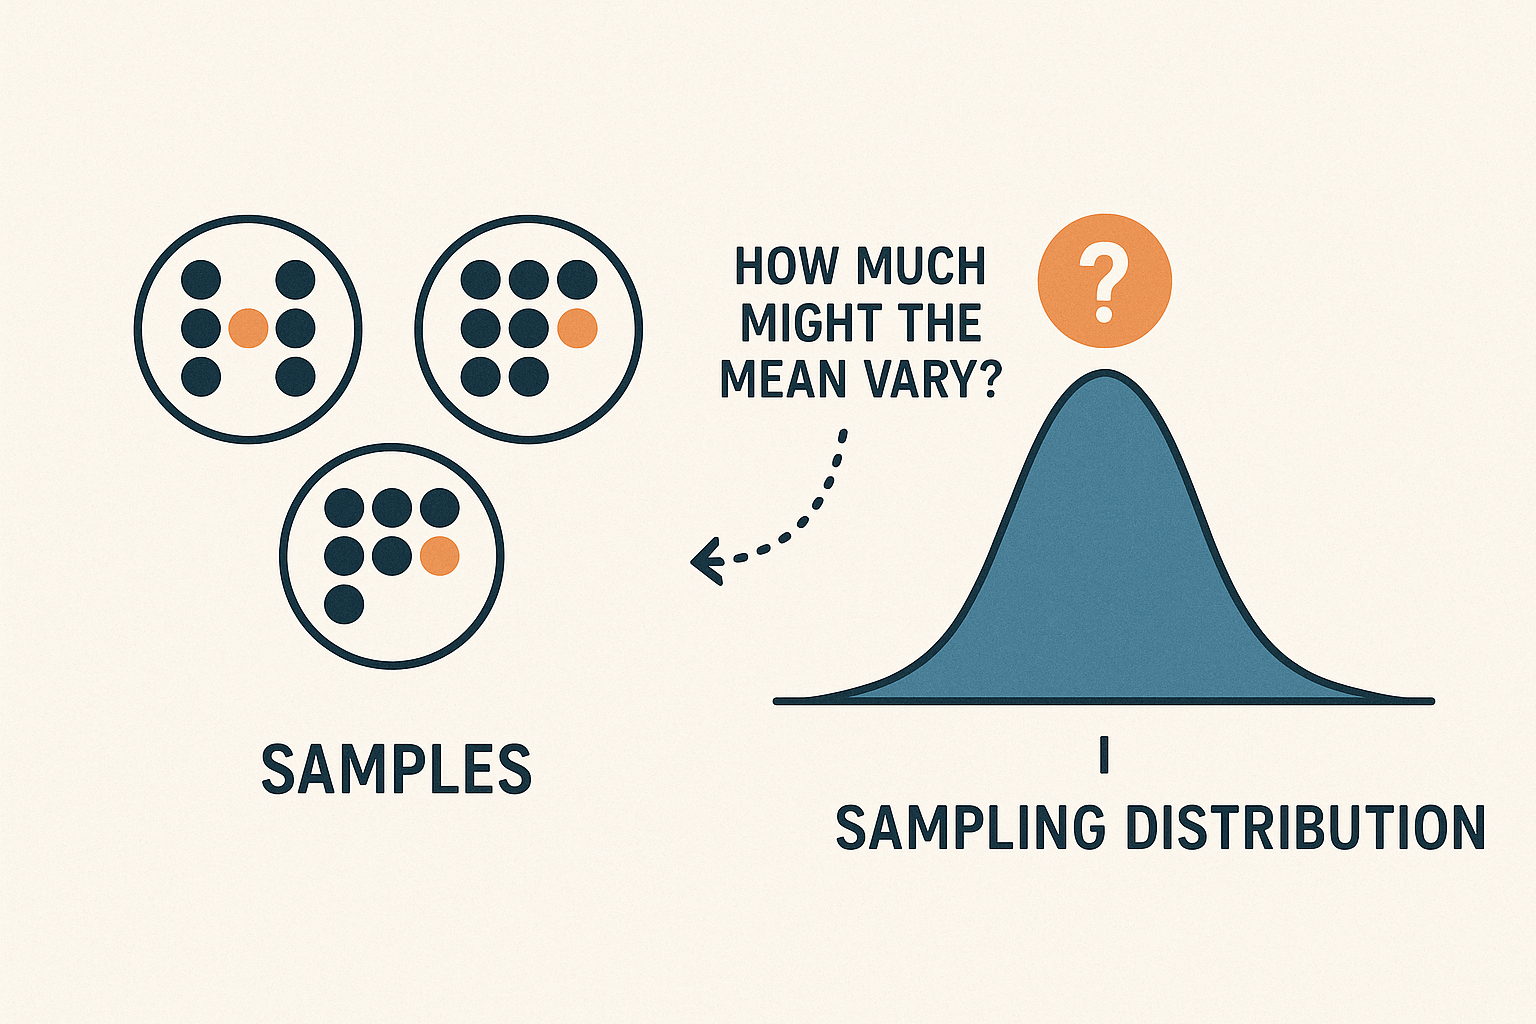
\includegraphics[width=\textwidth]{figures/s06_1_7.0x3.4.png}
    \end{column}
  \end{columns}
\end{frame}

%---------------------------------------------------------------------
%  05 Sampling Distributions
%---------------------------------------------------------------------
\begin{frame}{\numbadge{05}\ \ Sampling Distributions}
  \begin{keybox}[Definition]
    The distribution of a statistic across \textbf{all possible samples}.
  \end{keybox}
  \vspace{0.4em}
  \begin{columns}[T]
    \begin{column}{0.5\textwidth}
      \textbf{\color{qrnavy}Key Properties}
      \begin{itemize}
        \item \textbf{Sampling Variability:} statistics vary across samples
        \item \textbf{Bias:} does the statistic center on the true parameter?
        \item \textbf{Variability:} how spread out are the sample statistics?
      \end{itemize}
    \end{column}
    \begin{column}{0.5\textwidth}
      \textbf{\color{qrnavy}Managing Quality}
      \begin{itemize}
        \item Reduce \textbf{bias} $\rightarrow$ use random sampling
        \item Reduce \textbf{variability} $\rightarrow$ increase sample size
      \end{itemize}
    \end{column}
  \end{columns}
\end{frame}

%---------------------------------------------------------------------
%  06 Key Theorems  (EMBED LLN + CLT figure)
%---------------------------------------------------------------------
\begin{frame}{\numbadge{06}\ \ Key Theorems}
  \begin{columns}[T]
    \begin{column}{0.46\textwidth}
      \textbf{\color{qrnavy}1. Law of Large Numbers}\\
      Sample mean approaches the population mean as $n$ increases:
      \[ \bar{x}_n \rightarrow \mu \]
      \textbf{\color{qrnavy}2. Central Limit Theorem}\\
      Sample means become normally distributed as $n$ increases.
      \vspace{0.3em}
      \begin{keybox}[68--95--99.7 Rule]
        \small $68\%$ within $1\sigma$, $95\%$ within $2\sigma$, $99.7\%$ within $3\sigma$.
      \end{keybox}
    \end{column}
    \begin{column}{0.54\textwidth}
      \centering
      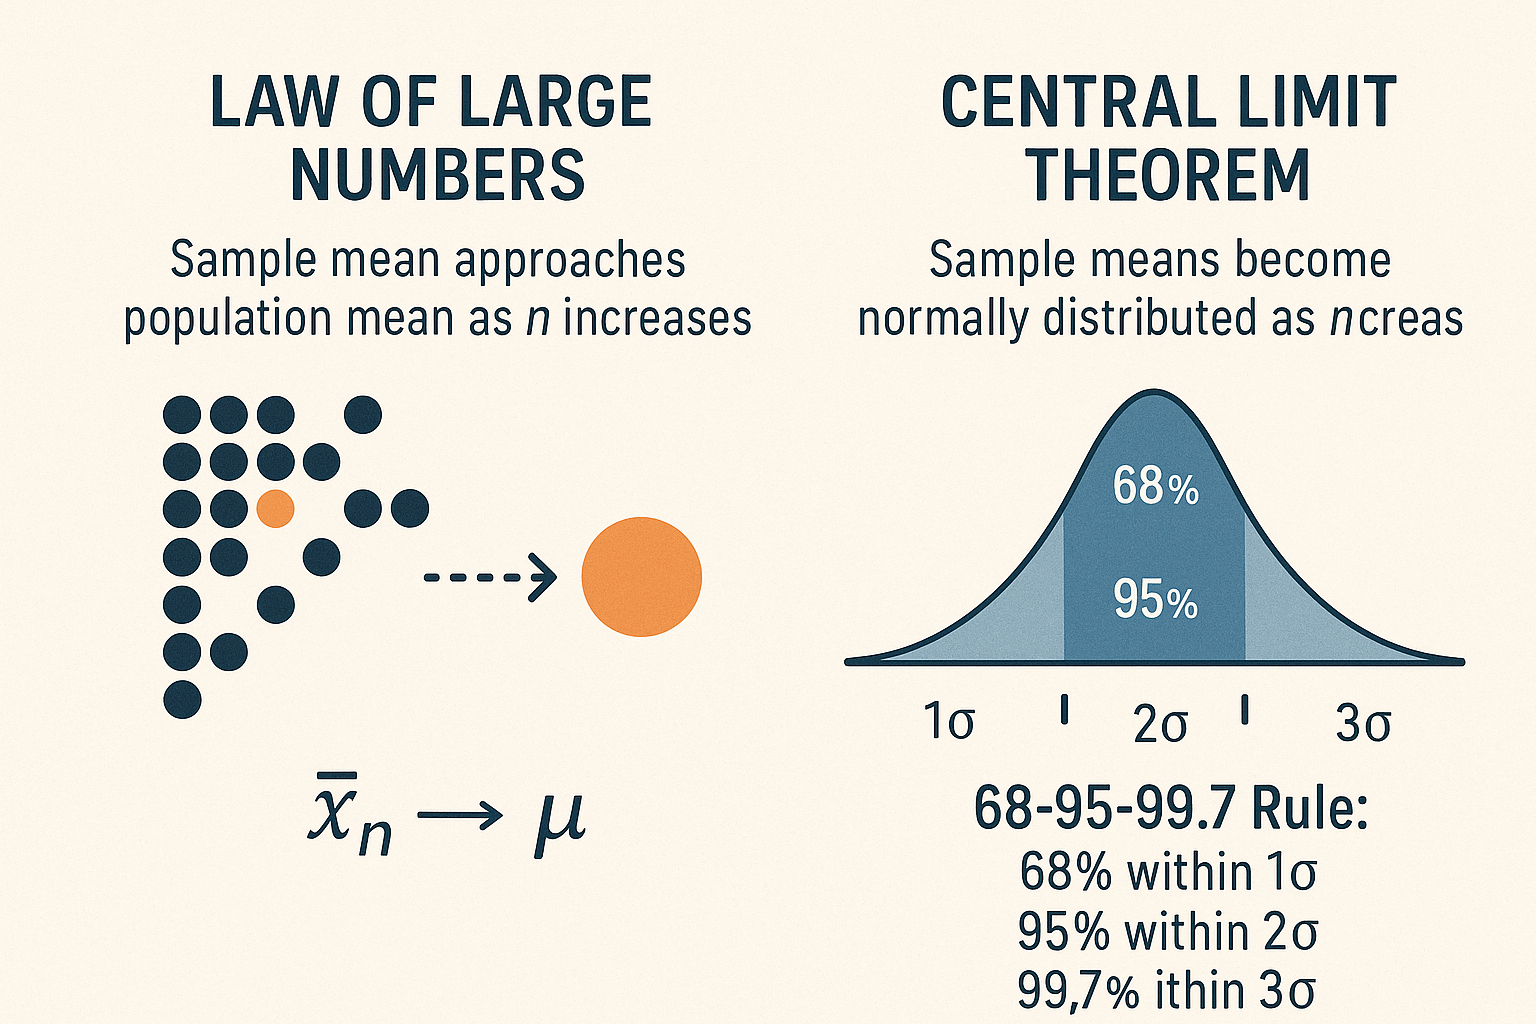
\includegraphics[width=\textwidth]{figures/s08_1_3.7x5.1.png}
    \end{column}
  \end{columns}
\end{frame}

%---------------------------------------------------------------------
%  Transition to RStudio
%---------------------------------------------------------------------
{\setbeamertemplate{footline}{}
\begin{frame}
  \vfill
  \centering
  {\color{qrnavy}\Huge\bfseries RStudio Practice}\\[0.8em]
  {\color{qrblue}\large Problem Set 2 with the \texttt{gapminder} Data}\\[0.4em]
  {\color{qrgray} See \texttt{Lab5.Rmd} / \texttt{Lab5\_1001.R}}
  \vfill
\end{frame}
}

\end{document}
